

Dados dos conjuntos $A$ y $B$, el conjunto unión de estos, que denotaremos
por $A \cup B$ y se leerá como ``$A$ unión $B$'', es el conjunto de
elementos que pertenecen a al menos uno de estos dos. Es decir,

\[ A \cup B = \{x \st x \in A \ \text{o} \ x \in B\} \]

\noindent o, con notación más propia de la lógica,

\[ A \cup B = \{x \st (x \in A) \lor (x \in B)\} \]

\noindent Recuerde que, tal y como se explicó antes, en la lógica, cuando se
usa la disyunción \emph{o}, sin especificar, nos referimos a la inclusiva;
no a la exclusiva.

En particular, si $A$ y $B$ son subconjuntos del conjunto $U$ y están
definidos por comprensión, es decir,

\begin{center}
\begin{tabular}{lr}
  $A = \{x \in U \st P_x\}$
    & $B = \{x \in U \st Q_x\}$
\end{tabular}
\end{center}

\noindent se tiene entonces que

\[ A \cup B = \{x \in U \st P_x \lor Q_x\} \]

\begin{example}
  1. Si los conjuntos son

  \begin{align*}
    A &= \{a, b, c, d\} \\
    B &= \{1, 2, 3, 4, 5, 6\}
  \end{align*}

  \noindent entonces

  \begin{align*}
    A \cup B = \{a, b, c, d, 1, 2, 3, 4, 5, 6\}
  \end{align*}

  2. Dados los conjuntos

  \begin{align*}
    C &= \{x \in \nset \st x \ \text{es múltiplo de} \ 4\} \\
    D &= \{x \in \nset \st x \ \text{es múltiplo de} \ 6\} \\
  \end{align*}

  \noindent se tiene

  \begin{align*}
    C \cup D = \{x \in \nset \st x \ \text{es múltiplo de} \ 4 \ \text{o de}
      \ 6\}
  \end{align*}

  3. La función real $f(x) = \sqrt{x^2 - 1}$ está definida en el conjunto

  \[ \{x \in \rset \st x^2 - 1 \geq 0\} \]

  Recuerde cómo se opera con desigualdades en ecuaciones. La desigualdad que
  se usa como predicado para definir el conjunto es $x^2 - 1 \geq 0$.
  Operando con esta,

  \begin{align*}
    x^2 - 1 &\geq 0 \\
    x^2 &\geq 1 \\
    \sqrt{x^2} &\geq \sqrt{1} = 1 \\
    |x| &\geq 1 \\
  \end{align*}

  \noindent y, como sabemos, la desigualdad $|x| \geq 1$ es lo mismo que el
  conjunto $({-\infty}, {-1}] \cup [1, \infty)$, que es el conjunto de
  valores en los que está definida la función. Puede comprobarse al observar
  su gráfica, en la figura~\ref{fig:dominio-func-1}. Debería fijarse en las
  proyecciones perpendiculares sobre el eje $X$ de la gráfica.

  % TODO Corregir el problema de incompatibilidad entre el Spanish de Babel
  % y TikZ. Quizás, pasarme a Polyglossia. También, pasar las dos figuras a
  % una minipage, pero me da un error.

  \begin{figure}
    \centering
    \foreignlanguage{english}{% Cambio de idioma por error del paquete Babel
    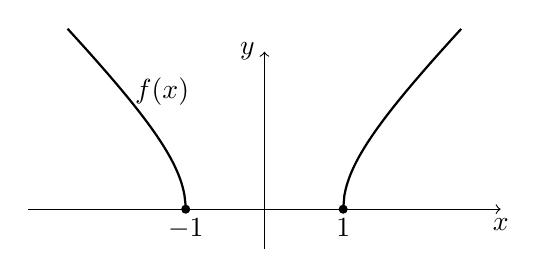
\begin{tikzpicture}[scale=1]
      % Ejes
      \draw[->] (-3,0) -- (3,0) node[below] {$x$};
      \draw[->] (0,-0.5) -- (0,2) node[left] {$y$};

      % Resaltado del dominio en el eje X
      % \draw[very thick] (-3,0) -- (-1,0); % Interval x <= -1
      % \draw[very thick] (1,0) -- (3,0);  % Interval x >= 1

      % Gráfica de la función
      \draw[thick, domain=-2.5:-1, samples=100] plot (\x, {sqrt((\x)^2-1)});
      \draw[thick, domain=1:2.5, samples=100] plot (\x, {sqrt((\x)^2-1)});

      % Puntos marcados
      \filldraw (-1,0) circle (0.05cm) node[below] {$-1$};
      \filldraw (1,0) circle (0.05cm) node[below] {$1$};

      % Etiqueta de la función
      \node at (-1.3,1.5) {$f(x)$};
    \end{tikzpicture}
    } % Fin del cambio de idioma
    \caption{Dominio de la función $f(x) = \sqrt{x^2 - 1}$.}%
    \label{fig:dominio-func-1}
  \end{figure}

  % TODO El siguiente no llego a entenderlo del todo.

  4. Teniendo en cuenta que $x^2 - y^2 = (x - y)(x + y)$, el conjunto $A =
  \{(x, y) \in \rset^2 \st x^2 - y^2 = 0\}$ de los puntos del plano
  $\rset^2$ es la unión de los conjuntos

  \begin{align*}
    A_1 &= \{(x, y) \in \rset^2 \st x - y = 0\} \\
    A_2 &= \{(x, y) \in \rset^2 \st x + y = 0\} \\
  \end{align*}

  \noindent es decir, el par de rectas de ecuaciones $y = x$ e $y = {-x}$,
  representadas en la figura~\ref{fig:dominio-func-2}.

  \begin{figure}
    \centering
    \foreignlanguage{english}{% Cambio de idioma por error del paquete Babel
    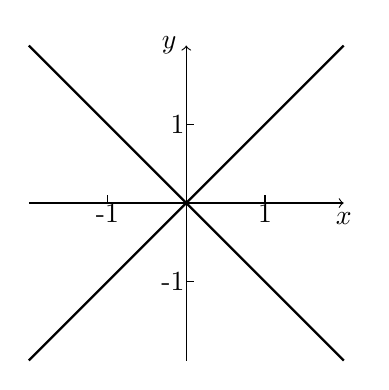
\begin{tikzpicture}[scale=1]
      % Ejes coordenados
      \draw[->] (-2,0) -- (2,0) node[below] {$x$};
      \draw[->] (0,-2) -- (0,2) node[left] {$y$};

      % Líneas asociadas a x^2 - y^2 = 0
      \draw[thick] (-2,-2) -- (2,2);   % Línea y = x
      \draw[thick] (-2,2) -- (2,-2);   % Línea y = -x

      % Marcas en los ejes (opcional)
      \foreach \x in {-1, 1} {
        \draw (\x,0) -- (\x,0.1) node[below] {\x};
        \draw (0,\x) -- (0.1,\x) node[left] {\x};
      }
    \end{tikzpicture}
    } % Fin del cambio de idioma
    \caption{Conjunto A = $\{(x,y) \in \rset^2 \st x^2 - y^2 = 0\}$}%
    \label{fig:dominio-func-2}
  \end{figure}
\end{example}





\subsubsection{Propiedades}

La unión de conjuntos tiene las propiedades siguientes, que se deducen
fácilmente de la definición. Cualesquiera que sean los conjuntos $A$, $B$ y
$C$, se tiene:

\begin{itemize}
  \item $A \subseteq A \cup B$ y $B \subseteq A \cup B$.
  \item $A \cup B = B \cup A$. (Propiedad conmutativa.)
  \item $A \cup (B \cup C) = (A \cup B) \cup C$. (Propiedad asociativa.)
  \item $A \cup \emptyset = A$
  \item $A \cup A = A$
\end{itemize}

\begin{exercise}
  Demuestre que para dos conjuntos cualesquiera $A$ y $B$ se cumple

  \[ A \cup B = B \quad \text{si y solo si} \quad A \subseteq B \]

  Demostraremos la igualdad mediante la doble implicación.

  Primero, se desea demostrar que, si $A \cup B = B$, entonces $A \subseteq
  B$. Por un lado, se cumple, tal y como se dice en la primera de las
  propiedades anteriores, que $A \subseteq A \cup B$.

  Además, como se da por hipótesis que $A \cup B = B$, concretamente se dará
  que $A \cup B \subseteq B$.

  Tal y como se vio, para la operación inclusión de conjuntos, $\subseteq$,
  se cumple la propiedad transitiva, con lo que podemos ``encadenar'' estas
  dos proposiciones que hemos obtenido, teniendo $A \subseteq B$, como
  deseábamos demostrar.

  Recíprocamente, supongamos que se cumple que $A \subseteq B$. Hay que ver
  solamente que $A \cup B \subseteq B$, pues $B \subseteq A \cup B$ es
  cierta por una de las propiedades de antes.

  Todo elemento $x \in A \cup B$ es elemento de al menos uno de los dos
  conjuntos $A$ y $B$. Si $x \in B$, ya habríamos terminado, pues es lo que
  deseamos demostrar. Si, por el contrario, se da que $x \in A$, entonces $x
  \in B$ ya que es la hipótesis de la que partimos, $A \subseteq B$. Por
  tanto, todo elemento de $A \cup B$ es elemento de $B$, o, lo que es lo
  mismo, $ A \cup B \subseteq B$.
\end{exercise}




